\chaptertoc{}


\vspace{1em}

In the last two decades, spectroscopy became one of the most powerful
techniques to survey galaxies across the Universe. 
Particularly thanks to its capability to obtain precise galaxy redshifts, 
spectroscopy allows us to build precise maps of the distribution 
of matter in three dimensions. 

This chapter is an overview on how to observe galaxies with 
spectroscopy and how the data is treated from the target selection 
all the way to the redshifts. 
I expose my work on improving the spectroscopic
data reduction pipeline for the extended Baryon Oscillation 
Spectroscopic Survey (eBOSS), for which I was the \emph{Lead Data Scientist}
for 3 years. 

Naturally, this chapter will 
focus on the spectroscopic observations with the 
Sloan Digital Sky Survey (SDSS), but the majority of the 
concepts introduced here also apply to the Dark Energy 
Spectroscopic Instrument (DESI). 


\section{Selecting the objects to observe}
\label{spectro:target}

The first step in building a fibre-based spectroscopic survey is to pre-select the objects to be observed. 
This step, known as \emph{target selection}, is required since one needs to know where to point 
the optical fibres that take the light from the objects to the spectrographs.
Therefore, we cannot simply observe all objects in a given field, we need to choose which targets to observe.

For the target selection, a prior \emph{photometric or imaging} 
survey is required. In the first years of SDSS, a photometric
survey was carried out, covering more than 
14~555 deg$^2$ of the sky \cite{yorkSloanDigitalSky2000}. 
The focal plane was equipped with six rows of five 
charge-coupled devices (CCD), each one covered with one of 
the SDSS filters: \textit{u, g, r, i} or \textit{z} 
\cite{gunnSloanDigitalSky1998, doiPhotometricResponseFunctions2010}.
A technique named drift-scanning was used to continuously observe 
``stripes'' of constant declination during the night.
The SDSS was the first of its kind to produce a systematic survey 
of the Universe in the optical domain, including data releases to the community.


Images were reduced using the SDSS photometric pipeline 
\cite{luptonSDSSImagingPipelines2001, padmanabhanImprovedPhotometricCalibration2008}. 
Fluxes/magnitudes and their uncertainties 
were computed for each detected object in five colour bands. 
Based on their fluxes and angular sizes relative to the 
point-spread function (PSF), each object received a 
photometric classification as star or galaxy.

The final list of objects with their respective fluxes and 
angular positions is the input for targeting algorithms. 
These algorithms aim to select a given type of object for 
spectroscopic follow-up, based solely on their fluxes and colours. 
For galaxy surveys, it is vital to be able to distinguish between 
galaxies - the objects of our interest - and stars - which belong
to our own galaxy and have a distinct scientific purpose.
Additional colour cuts also help selecting a given redshift range 
for particular types of galaxies. 

Since we are interested in the clustering of 
galaxies, it is essential to obtain a relatively 
homogeneous angular density of targets so to avoid spurious 
correlations. Target selection algorithms enforce a requirement
of about 15 per cent on the fluctuations of the angular number density 
of targets. Residual fluctuations have to be corrected before
any clustering measurements. 
I will discuss further about this issue in section~\ref{galaxies:catalogue}. 

Table~\ref{tab:target_selection} provides a summary of target selection
algorithms for several types of galaxy types and redshift ranges. 

\begin{table}
    \small
    \centering
    \caption{Surveys and their target selection algorithms}
    \label{tab:target_selection}
    \begin{tabular}{lcl}
    \hline 
    \hline
        Sample & Redshift range & Reference \\
    \hline 
    SDSS MGS & $0.0 < z < 0.2$ & \cite{straussSpectroscopicTargetSelection2002} \\
    BOSS LOWZ galaxies & $0.2 < z < 0.4$ &  \cite{reidSDSSIIIBaryonOscillation2016} \\
    BOSS CMASS galaxies  & $0.4 < z < 0.7$ & \cite{reidSDSSIIIBaryonOscillation2016} \\
    BOSS \lya forest quasars & $2.0 < z < 3.5$ & \cite{rossSDSSIIIBaryonOscillation2012} \\
    eBOSS LRGs & $0.6 < z < 1.0$ & \cite{prakashSDSSIVExtendedBaryon2016} \\
    eBOSS ELGs  & $0.7 < z < 1.1$ & \cite{raichoorSDSSIVExtendedBaryon2017} \\ 
    eBOSS quasars as tracers & $0.8 < z < 2.2$ &  \cite{myersSDSSIVExtendedBaryon2015} \\
    eBOSS \lya quasars & $2.0 < z < 3.5$ &  \cite{myersSDSSIVExtendedBaryon2015} \cite{palanque-delabrouilleExtendedBaryonOscillation2016} \\
    DESI BGS & $0.0 < z < 0.6$ & \cite{hahnDESIBrightGalaxy2022} \\
    DESI LRGs & $0.4< z < 1.0$ & \cite{zhouTargetSelectionValidation2022} \\
    DESI ELGs & $0.6 < z < 1.6$ & \cite{raichoorTargetSelectionValidation2022} \\ 
    DESI quasars & $0.5 < z < 4.0 $ & \cite{chaussidonTargetSelectionValidation2022} \\
    \hline 
    \hline
    \end{tabular}
\end{table}

\section{Pointing fibres to the sky}
\label{spectro:fibres}

Once the targets are chosen, we need to define the observing strategy
for spectroscopy. This strategy is defined based on several constraints, 
such as 
\begin{itemize}
    \item the focal plane dimensions, which is a one meter diameter plate holding 1000 optical fibres;
    \item the field of view of the telescope, which is about 5 deg$^2$ for the plates; 
    \item the number of fibres. There are a total of 1000 available fibres  of 
            which 80 are used for sky observations and 20 for standard stars; 
    \item the size of the extragalactic footprint, which is roughly 10 000 deg$^2$; 
    \item the fibre completeness, i.e., the fraction of targets receiving an 
          optical fibre. The completeness has to be usually above a certain 
          threshold over all the footprint;
    \item exposure times and total observing time available. 
        Exposure times are dependent on the average signal-to-noise ratio of 
        the observed targets, which need to reach a certain threshold. 
        The total observing time of the program is roughly four to five years. 
    \item visibility window of a given patch of the sky at a given time of the year; 
    \item priority for fibre assignment. Some types of targets have higher priority than others,
        which affects the fibre completeness of the low-priority samples.  
\end{itemize}

The process of dividing the sky into overlapping projections of the focal plane 
is called \emph{tiling}. A detailed description of the tiling algorithm can be found in 
\cite{blantonEfficientTargetingStrategy2003}. 
Once  the tiling and fibre assignment
are set, this information is sent to the plate production and drilling of holes 
that will hold the optical fibres. Focal plane plates are drilled a few months 
before observing and are unique for a particular patch of the sky and observing time. 
Not observing the plate at the designed hour angles causes loss of flux due to increased absorption and 
refraction by the atmosphere. 

The drilled plates are sent to the Apache Point Observatory (APO) in New Mexico
where the Sloan 2.5-meter Telescope is based. On the mountain, 
observers attach the plates into cartridges that will fit at the focal plane of the
telescope. There are about 15 cartridges, each equipped with 1000 optical fibres.
The fibres are plugged by hand, by one or two observers during the afternoon preceding 
the observation night. Plates are unplugged from their cartridge once a sufficient
number of exposures has been taken. A minimum of 3 exposures are taken per plate.
Figure~\ref{fig:cartridge} shows an illustration of a cartridge with the focal plane 
plate on top.

\begin{figure}
    \centering 
    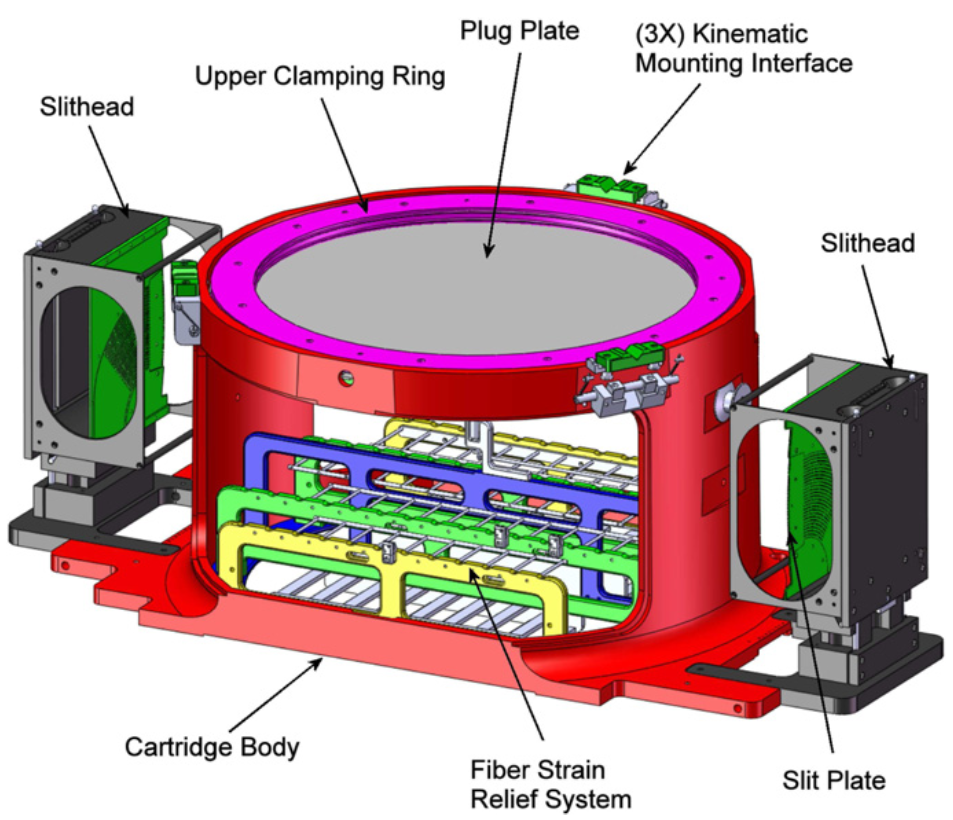
\includegraphics[width=0.7\textwidth]{fig/spectro/cartridge.png}
    \caption{Illustration of the SDSS cartridge holding the focal plane plate and the optical fibres. 
    Figure extracted from \cite{smeeMultiobjectFiberfedSpectrographs2013}. }
    \label{fig:cartridge}
\end{figure}
 
The light of the objects is transported by the optical fibres through the 
Sloan spectrographs, shown in Figure~\ref{fig:spectrograph}. 
There are two spectrographs attached at the focal plane
of the telescope. Each spectrograph receives the light from 500 fibres and passes 
it through a beam-splitter, dividing it into a red and blue channels. 
Each channel has is own grism that spreads the light over wavelength before
hitting the CCDs. The blue camera observes roughly from 3500 to 6000~\angstrom\ and the red
camera from 6000 to 10500~\angstrom. The resolution $R \equiv \lambda / \Delta \lambda$ 
increases with wavelength from 1500 to 2000 on the blue camera and from 2000 to 2500 
on the red camera. 

\begin{figure}
    \centering 
    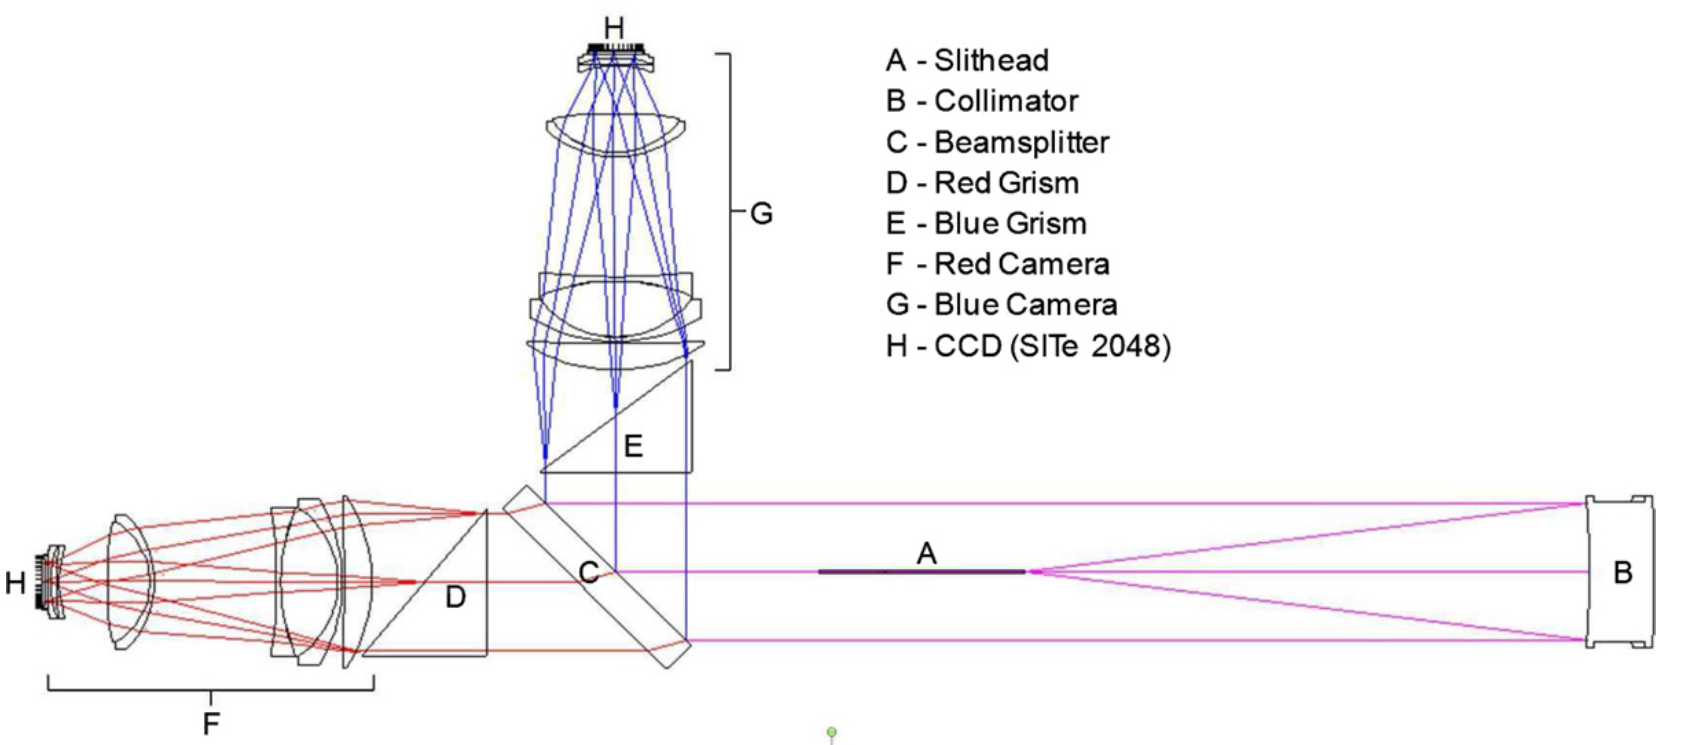
\includegraphics[width=\textwidth]{fig/spectro/spectrograph.png}
    \caption{Illustration of one SDSS spectrograph. 
    Light propagates from the slithead (also shown in Figure~\ref{fig:cartridge})
    towards the blue and red cameras. 
    Figure extracted from \cite{smeeMultiobjectFiberfedSpectrographs2013}. }
    \label{fig:spectrograph}
\end{figure}
 

In addition to the science exposures (observing galaxies), a small set
of calibration exposures is also taken, typically at the beginning and at the end 
of the observing run. Flat exposures are taken with lamps that emit over all 
wavelengths. The light is passed through the spectrographs, so we refer to these
as fibre-flats, as opposed to the exposures taken without the spectrographs, named 
super-flats. With another type of lamp, which emit narrow lines at some specific 
wavelengths, arc exposures are obtained, that are used to derive the relation between 
wavelength and CCD pixel location.

\section{From electrons to spectra}
\label{spectro:pipeline2d}

This section describes the data reduction pipeline of 
spectroscopic observations by the SDSS telescope, for which 
I contributed as the eBOSS Lead Data Scientist. 
This automated pipeline transforms the counts stored in CCDs into 
calibrated spectra, for which redshifts are estimated. 
Figure~\ref{fig:pipeline} displays a flowchart of the process. 
The software, named \texttt{idlspec2d}, was written in Interactive Data Language (IDL)
and can be found online\footnote{\url{https://svn.sdss.org/public/repo/eboss/idlspec2d/tags/v5_13_0/}}.
The latest version used in Data Release 16 
of eBOSS data is \texttt{v5\_13\_0} (\cite{ahumada16thDataRelease2020}).


\begin{figure}
    \centering 
    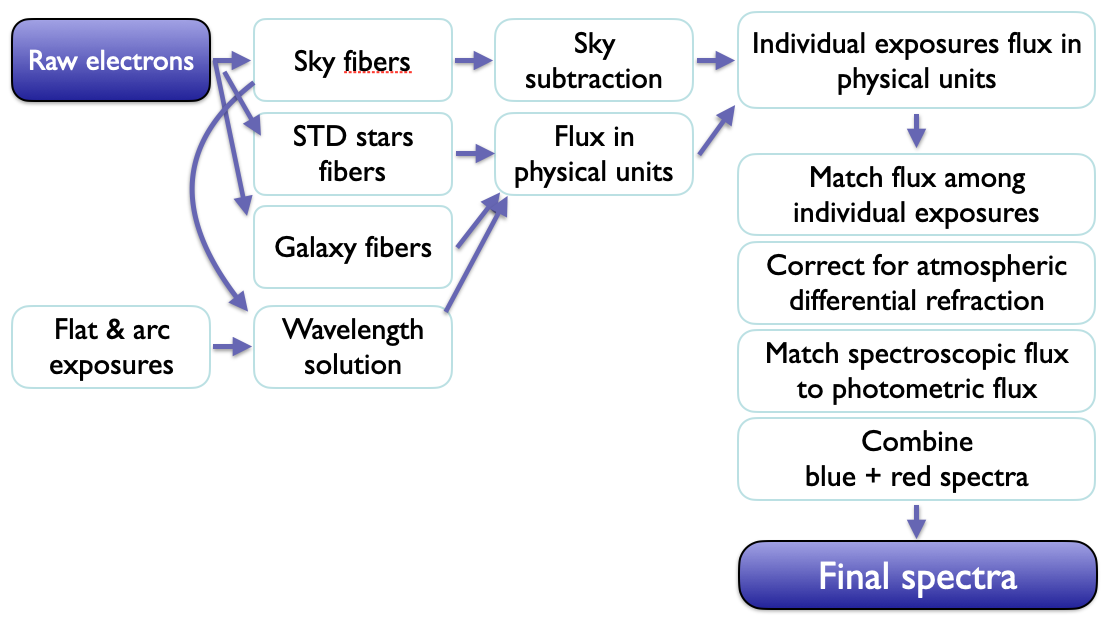
\includegraphics[width=\textwidth]{fig/spectro/pipeline_flowchart.png}
    \caption{Flowchart summarising the several steps of the automated data reduction pipeline from SDSS spectroscopic data.}
    \label{fig:pipeline}
\end{figure}
 

The dispersed light of each object falls onto CCD detectors containing 
2048x2048 square 24$\mu$m pixels. 
There are 500 traces per CCD, except when fibres are broken or unplugged by accident. 
The traces of each spectra are parallel and slightly curved towards the edges. 
They are separated by about 7 pixels. 

The first step of the data reduction is to remove bias and dark, mask 
cosmic rays and other known bad pixels, 
convert counts into electrons using estimated gain values, 
and correct for the super-flat image (flat taken without the spectrograph). 

The next step is to extract the total number of counts per wavelength and per object.
One of the axis of the CCD is aligned with the wavelengths, but we do not know the
wavelength solution at this point. The other axis is aligned with fibre number. 
The extraction of the fluxes is performed by bundles of 20 fibres. A set of 20 Gaussian
profiles plus a third order polynomial term are fit simultaneously over the counts. 
From the best-fit parameters of the Gaussian, one can compute the total flux at each 
wavelength for each object. This fit is performed regardless of whether the fibres contain 
flux from sky, stars or galaxies. 
The extraction step is performed similarly to science, flat and arc exposures. 


One important aspect of extraction is: what do we use as weights in the fit?
For SDSS-II and III, the extraction used the total estimated variance of each pixel,
assumed to be Poisson with mean equal to the number of observed hits in the pixel. 
However, in SDSS-IV eBOSS we pushed the limits of the instrument by observing fainter
objects. In this regime, we started to observe biases due to this weighting scheme in 
the extraction. The ideal extraction would use the true variance 
(\cite{horneOptimalExtractionAlgorithm1986}), not the estimated
one, as a weight. Using the estimated one yields a bias in the final fluxes. 
We modified the extraction algorithm such that it would use a flux-independent weight 
for the fit, yielding unbiased fluxes. Consequently, this extraction is less 
optimal, yielding slightly larger flux uncertainties. Biased fluxes affected 
particularly the analysis of \lya forests, as described in chapter~\ref{chap:forests}
or in the appendix of \cite{bautistaMeasurementBaryonAcoustic2017}.

The fibre-flat images are used to calculate the traces positions and widths 
(more precisely than in science images) 
and to correct for throughput variations across fibres. 
The arc images are used to calculate the wavelength solution and 
the dispersion in the wavelength direction based on the line widths. 
Sky lines in science exposures are eventually used to do small adjustments 
to the arc-image solution. 

The flux in the sky fibres are used to fit a sky model in units of counts.
A polynomial dependency over fibre index is used to account to variations 
over the focal plane. This sky model is then subtracted from all science 
spectra, including the sky spectra themselves and calibration stars. 
The sky-subtracted sky fibres are a good metric to evaluate the quality of 
sky subtraction algorithm. 

The next step of the reduction is the \emph{flux calibration}, 
which converts the observed counts into flux in physical units. 
The spectra of standard stars are the main ingredient of the flux calibration. 
The stars chosen for calibration are of type F, with small variations in 
temperature and metallicity. Physical models of their spectral emission 
including absorption features can be obtained via complex stellar synthesis calculations. 
The goal is to fit absorption lines to the data 
in order to determine the exact model for each observed star. 
We start by isolating the absorption lines in the observed spectrum 
(in units of counts) by fitting a smooth function over its shape, 
then dividing the whole spectrum by this model. 
This residual spectrum has only absorption features in an dimensionless scale.
The same is done for the physical stellar models. We fit these absorption features 
to all models to find the best star model for a given spectra.
Once the best-fit parameters of the star are found, 
a calibration vector is constructed by simply taking the ratio of 
the observed counts to the full model including its smooth component. 
A set of ten stars are fit independently and a single calibration 
vector is obtained from them. This final calibration vector is then 
applied to all other galaxy spectra in order to convert their number counts into
flux in physical units. During the last years of eBOSS, I updated 
the set of physical stellar models from the Kurucz catalogue to those used 
in DESI (\cite{allendeprietoCollectionModelStellar2018}) 
which have a larger diversity in stellar 
parameters and more precise absorption features. This update contributed
to a significant reduction of flux calibration residuals 
computed using stacks of spectral regions of quasars without emission 
or absorption lines. Figure~\ref{fig:flux_calibration_residuals} shows this 
improvement. 

\begin{figure}
    \centering
    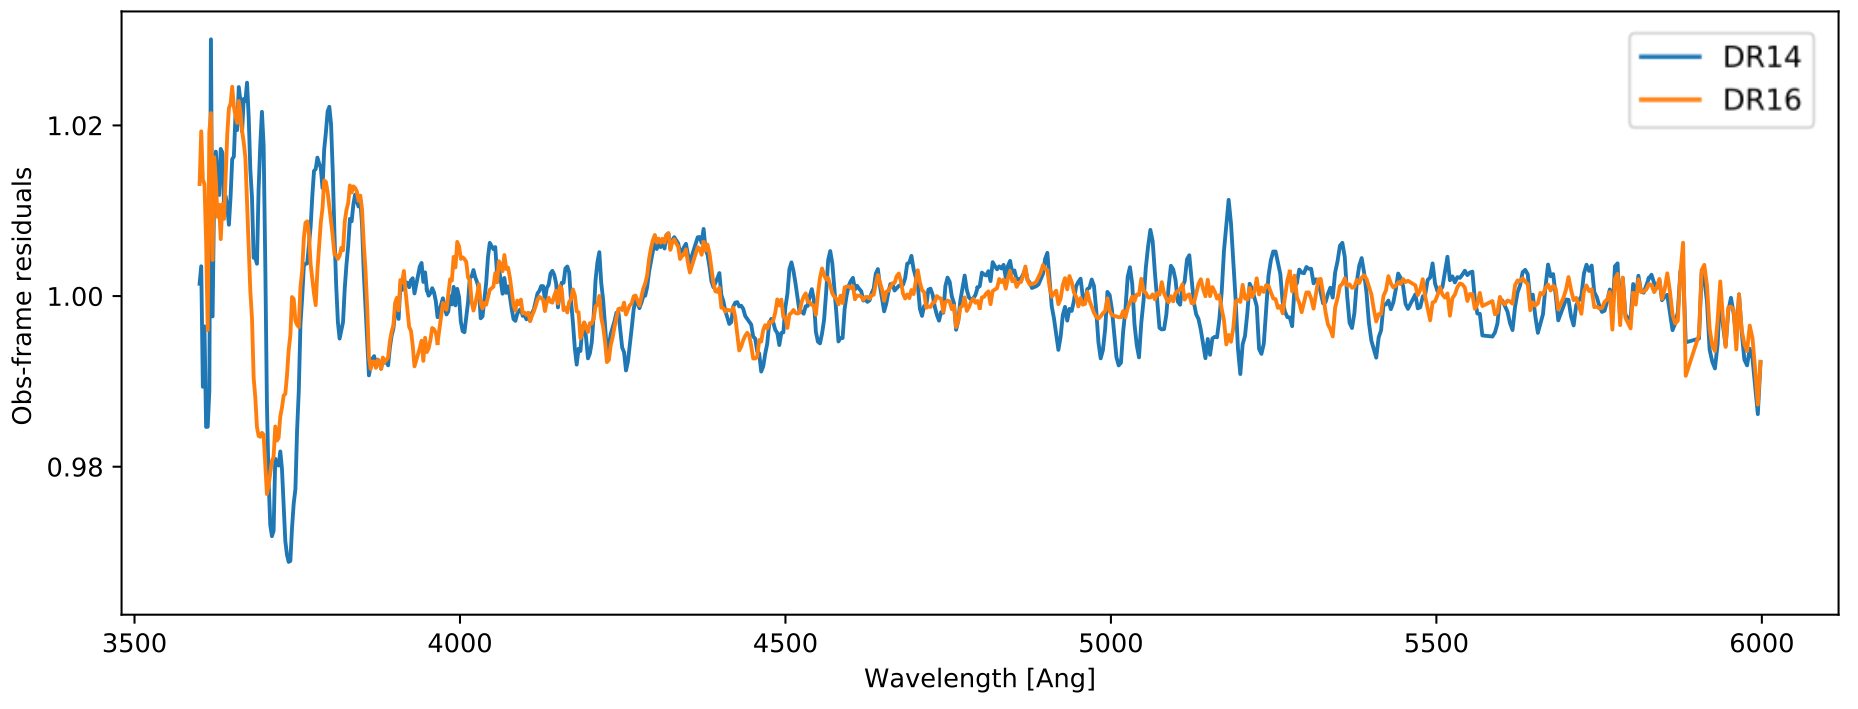
\includegraphics[width=\textwidth]{fig/spectro/picca_calibration_residuals_DR14_DR16_civ.png}
    \caption{Flux calibration residuals computed using an observer-frame stack of 
    quasar spectral regions without emission or absorption lines. 
    Two versions of the automated pipeline are displayed. The DR16 includes an 
    update of the stellar models used to fit spectra of standard stars. 
    We see a significant improvement in these residuals with this change. }
    \label{fig:flux_calibration_residuals}
\end{figure}

Once individual science exposures are converted into physical flux units, 
we proceed to the co-addition of these exposures into a single set of spectra. 
For a given object, a B-spline is fitted over all observed spectra, 
using a new wavelength grid with constant steps in $\log_{10} \lambda$ of $10^{-4}$. 
The best-fit spline is the final co-added spectrum for this object. 
The co-addition is made independently for each object. 
At this stage, we also combine spectra from blue and red cameras into 
one single spectrum covering the full wavelength range of 3500 to 10500 $\AA$. 
The last step of this process is the calculation of potential broadband 
distortions in flux caused by atmospheric differential refraction (ADR). 
Using information from the plate design, the position of the fibres in 
the plate and the actual observations (airmass, hour-angle), one can 
compute a correction vector that is also applied to all spectra. 

During the whole reduction, pixels or whole fibres can be masked due to any issues, 
or when the robustness of flux calculations is compromised. 
Each pixel has a flux and an uncertainty estimates. The latter is expressed 
as an inverse variance, which can be used directly as a weight in analyses.



\section{From spectra to redshifts}
\label{spectro:pipeline1d}

The next and last step of the automated data reduction pipeline is the 
spectral classification and redshift measurement. 
A set of physical templates of stars, galaxies and quasars is fit to 
each spectrum by a simple $\chi^2$ minimization. For each template, 
we scan over several values of redshifts to obtain the minimum $\chi^2$. 
The redshift ranges probed depend on the type of template: 
stellar templates are allowed to vary around $z =0$, 
galaxy templates are fitted over $0 < z < 2$ and quasar ones over $0 < z < 7$. 
The five best pairs of template and redshift producing the smallest $\chi^2$ values are stored. 
Redshift uncertainties are estimated using the $\chi^2$ profiles around the minima.
If the difference between the first and second best-fit $\chi^2$ values
is smaller than a certain threshold (corresponding to roughly 
5$\sigma$ for one parameter), a warning flag is set, meaning 
that the classification is not to be trusted. 
Figure~\ref{fig:spec1d} illustrates an example of $\chi^2$ profile versus redshift,
with the potential first and second best-fit redshifts and their uncertainty estimation. 

\begin{figure}
    \centering
    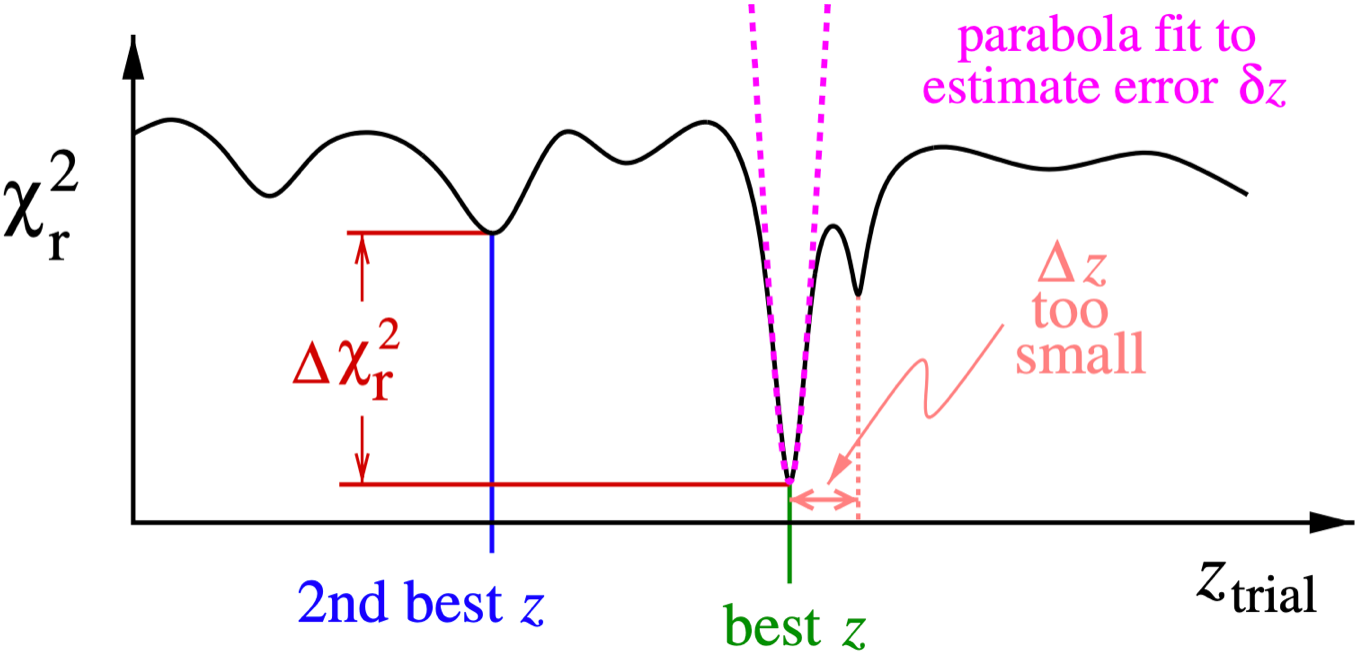
\includegraphics[width=0.7\textwidth]{fig/spectro/spec1d_chi2.png}
    \caption{Illustration of a $\chi^2$ profile for a spectral template versus redshift. 
    The best redshift is defined by the location of the global minimum (green). 
    Other minima separated by less than 1000~\kms are not considered to be separate (pink). 
    A parabolic fit to the global minimum (magenta) is used to determine redshift uncertainty. 
    The second-best redshift fit is determined by the location of the second-lowest well-separated minimum (blue). 
    The difference $\Delta \chi^2$ (red) between best and second-best fits is used 
    to quantify the confidence in the measurement.
    Figure extracted from \cite{boltonSpectralClassificationRedshift2012a}. }
    \label{fig:flux_calibration_residuals}
\end{figure}

A program of visual inspection of reduced spectra is carried out following the first observations 
of a new survey. 
Visual inspection is a important step in order to verify 
the quality of the data reduction, the automated classification and the redshift measurement. 
A truth table containing the visually confirmed redshifts and classifications
for thousands of spectra is one of the results of the visual inspection. 
This truth table is used to compute the actual density of tracers that are 
obtained for a given target selection, as a function of redshift. 
Spectral features caused by problems in the reduction were then reported to the
pipeline team. 

During the first months of eBOSS, I coordinated a program of 
visual inspection where about 15 members analysed about a thousand spectra each
(with some overlap for cross-checking). This provided a truth table
for the Luminous Red Galaxies from eBOSS. Similar programs were carried out
for the eBOSS Emission Line Galaxies and quasars. The inspections of eBOSS quasars
continued throughout the whole program, where a small fraction of
the spectra without confident automated classifications were inspected.
In DESI, a larger visual inspection program was put in place for the same goals.

This concludes the description of a spectroscopic survey: 
a machine converting photons to redshifts useful for cosmology.  